%%%%%%%%%%%%%%%%%%%%%%%%%%%%%%%%%%%%%%%%%%%%%%%%%%%%%%%%%%%%%%%%%%%%%%%%%%%
%
% Plantilla para un artículo en LaTeX en español.
%
%%%%%%%%%%%%%%%%%%%%%%%%%%%%%%%%%%%%%%%%%%%%%%%%%%%%%%%%%%%%%%%%%%%%%%%%%%%

\documentclass[11pt,twocolumn,spanish]{article}

% Esto es para que el LaTeX sepa que el texto está en español:
\usepackage[spanish]{babel}

% Paquetes de la AMS:
\usepackage{amsmath, amsthm, amsfonts}


\usepackage[utf8]{inputenc}
\usepackage{amsmath}
\usepackage{amsfonts}
\usepackage[spanish]{babel}
\usepackage{latexsym}
\usepackage{euscript}
\usepackage{graphicx}
\usepackage{tdclock}
\usepackage{enumerate} 
\usepackage{float}
\usepackage{multirow, array} 
\usepackage[latin1]{inputenc}
\usepackage{caption}
\usepackage[dvips]{graphicx}

% tamaño de hoja
\oddsidemargin 0.05in
\textwidth 6.3in
\topmargin -0.5in
\headheight 0in
\textheight 9in 

% Teoremas
%--------------------------------------------------------------------------
\newtheorem{thm}{Teorema}[section]
\newtheorem{cor}[thm]{Corolario}
\newtheorem{lem}[thm]{Lema}
\newtheorem{prop}[thm]{Proposición}
\theoremstyle{definition}
\newtheorem{defn}[thm]{Definición}
\theoremstyle{remark}
\newtheorem{rem}[thm]{Observación}

% Atajos.
% Se pueden definir comandos nuevos para acortar cosas que se usan
% frecuentemente. Como ejemplo, aquí se definen la R y la Z dobles que
% suelen representar a los conjuntos de números reales y enteros.
%--------------------------------------------------------------------------

\def\RR{\mathbb{R}}
\def\ZZ{\mathbb{Z}}

% De la misma forma se pueden definir comandos con argumentos. Por
% ejemplo, aquí definimos un comando para escribir el valor absoluto
% de algo más fácilmente.
%--------------------------------------------------------------------------
\newcommand{\abs}[1]{\left\vert#1\right\vert}

% Operadores.
% Los operadores nuevos deben definirse como tales para que aparezcan
% correctamente. Como ejemplo definimos en jacobiano:
%--------------------------------------------------------------------------
\DeclareMathOperator{\Jac}{Jac}

%--------------------------------------------------------------------------
\title{Caos}
\author{Oscar De la Cruz Echeveste\\
  \small Dept. Plantillas y Editores\\
  \small E12345\\
  \small España
}

\begin{document}
\maketitle

\abstract{Esto es una plantilla simple para un artículo en \LaTeX.}

\section{Introducción}
Galileo Galilei fue matemático y astrónomo italiano del siglo XVI y XVII, conocido por muchos por su icónica riña contra los miembros de la iglesia católica al tratar de mostrarles que algunos cuerpos celeste no giraban alrededor de la tierra, como el mismo lo pudo observar en el movimiento de las lunas Jovianas. Atrevimientos como este y sumado a su carácter necio y egocéntrico lo llevaron a la excomunión y al arresto domiciliario en 1633 hasta el día de su fallecimiento en 1642 a la edad de77 años. En el proceso en el que Galileo se adentro en la filosofía natural, observo la forma en que los cuerpos en movimiento evolucionaban a lo largo del tiempo y parecían obedecer ciertos patrones que eran predecibles al describirse en forma matemática. Tal fue su fascinación que dedico su vida a estudiar esta armonía que él encontraba en la naturaleza. “La matematica è la lingua in cui Dio ha scritto l'universo” es una de las frases que se le atribulen a Galileo y, aunque desconozco la veracidad de esta cita, es una frase bastante acertada. Por una extraña razón la naturaleza puede caracterizarse por modelos matemáticos con los cuales podemos predecir la evolución o cambios en el sistema con una envidiable precisión. En general, esta es la tarea a la que se adentra un físico. La matemática se vuelve la herramienta de trabajo más poderosa que da paz y tranquilidad a la certidumbre que caracteriza y predice la evolución de los sistemas. Pero la realidad es más complicada de lo que se espera. Ciertamente, la dinámica de muchos de los sistemas que se estudian no es tan sencilla de predecir. Uno se estos sistemas, y tal vez el de mayor antigüedad, es el problema de los tres cuerpos, el cual consta de tres objetos celestes en movimiento afectados por la gravedad de cada uno. Tanto Newton (1642-1727) como sus predecesores matemáticos han estudiado este problema por los últimos siglos. Fue el matemático francés Henri Poincaré (1854 - 1912) quien demostró que no había una solución analítica para este problema y agrego que esto representaba la naturaleza del caos. 

Poincaré fue un pionero en el estudio del caos, un concepto que hasta hoy en día parece ser desconocido para muchos, temido por algunos y apasionado para otros pero sin duda un dolor de cabeza para todo aquel estudioso de esta área. Trabajar con el caos significa trabaja con sistemas dinámicos no lineales, es decir, sistemas que cambian su estado en el tiempo basados en su estado inicial - la ecuación que los representa es de la forma $ \frac{dx}{dt} = f(x,t;\alpha)$ - y al ser no lineal significa que el sistema total no puede verse como la suma de su partes - la ecuación $ \frac{dx}{dt} = f(x,t;\alpha)$ que lo representa tiene una función $f(x,t;\alpha)$ no lineal -  . 

Los sistemas dinámicos pueden ser discretos y continuos.  Los sistemas discretos toman el paso del tiempo como cantidades de números enteros, por ejemplo la ecuación $x_{n+1} = mx_{n}(1-x_{n})$ muestra como evoluciona $x$ conforme el tiempo, en este caso  $n$, avanza en una unidad. En cambio, los sistemas dinámicos discretos se expresan como ecuaciones diferenciales $\frac{dx}{dt} = mx(1-x)$ donde, de nuevo x cambia en el tiempo pero de forma infinitesimal. En el presente texto se mostraran ejemplo de ambos sistemas en el desarrollo de los temas. 

Aquí va el texto.
\begin{equation}\label{eq:area}
  S = \pi r^2
\end{equation}
Uno puede referirse a ecuaciones así: ver ecuación (\ref{eq:area}).
También se pueden mencionar secciones de la misma forma: ver sección
\ref{sec:nada}. O citar algo de la bibliografía: \cite{Cd94}.

\section{Mapeo}\label{sec:nada}

En matemáticas un mapeo, aplicación o  función es una regla que asocia valores de algún conjunto que llamaremos \textit{conjunto objeto} \textbf{A} a un \textit{conjunto objetivo} \textbf{B}. Podemos representar esto de manera gráfica como:

\begin{equation*}
\begin{split}
&f:  A \longrightarrow B \\
&a  \mapsto f(a) = b  
\end{split}
\end{equation}

Donde $f$ es la regla de asociación entre los valores del conjunto A (en este caso a)  a los valores del conjunto B (en este caso b). Un ejemplo sencillo es una función $f:  \mathbb{R} \longrightarrow \mathbb{R} $ tal que $x \mapsto f(x) = 2x$ donde la función $f$ relacionas los elementos del conjunto de los números reales con los elementos de un conjunto igual de tal forma que cada elemento del conjunto objetivo es el doble de un sólo elemento del conjunto objeto. En la figura 2.1 se puede ver un ejemplo gráfico de un mapeo entre un conjunto de todas las pelotas deportivas y los números naturales \mathbb{N}. Este mapeo podría ser una regla como: “las pelotas de un sólo color tendrán el valor de uno, las pelotas de un dos colores tendrán el valor de dos, las pelotas de tres colores tendrán el valor de tres, … ”. 
\begin{figure}[H]
\centering
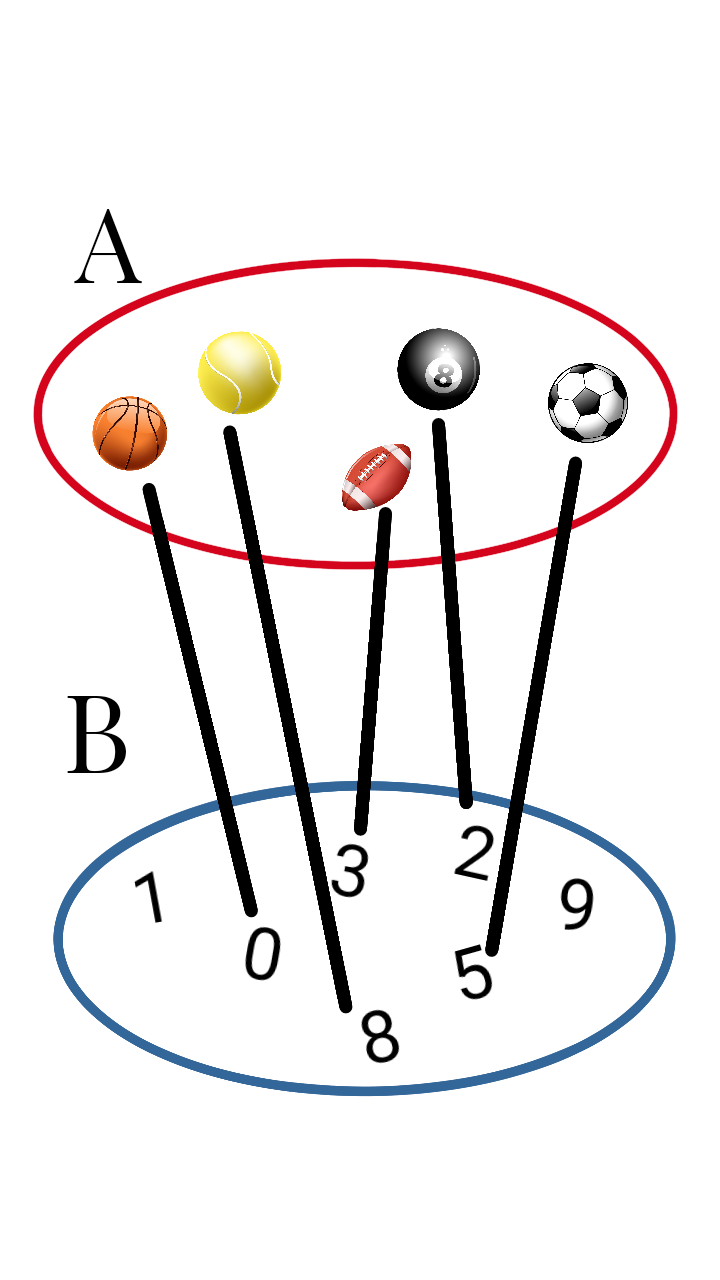
\includegraphics[width=3cm]{figura_1}
\caption*{\textbf{Figura 2.1}: Representación gráfica de un mapeo de conjuntos del pelotas deportivas al conjunto de números naturales $\mathbb{N}$ }
\label{etiqueta}
\end{figure}
\end{enumerate}
En la teoría de sistemas dinámicos los mapeos son usados para crear sistemas dinámicos discretos y así poder seguir su evolución. Esto se consigue usando mapeos iterativos los cuales se construyen en base a una función:
\begin{equation}
x_{n+1} = f(x_{n})
\end{equation}
Es decir, una función que depende de $x_n$  determinara el valor que tomara $x_{n+1}$ a travez de la aplicacion $f$ y este a su vez al evaluarse $f(x_{n+1})$ determinara el suficiente valor $x_{n+2}$.  Un ejemplo común para entender este proceso es el  \textbf{mapeo logístico}. Este proviene modelar el crecimiento para una población biológica y tiene la siguiente forma:
\begin{equation}\label{eq:log}
x_{n+1} = f_{A}(x_{n}) = Ax_{n} (1-x_{n})
\end{equation}
Para su construcción tomaremos el ejemplo de Robert C. Hilborn de su libro “Chaos and Nonlinear Dynamics: an introduction for scientists and engineers” \cite{Cd94}. Analizando la población de mariposas que nacen y mueren a lo largo de un año podemos saber que la cantidad de mariposas $N_{1}$ al terminar el año depende de la cantidad de estas que había al comenzar $N_{0}$ y ademas del entorno en el que viven. Este ultimo factor se incluye como un número $A$ de tal forma que si $A>1$ el número de mariposas crece y lo contrario si $A<1$ . De tal forma que tenemos la siguiente relación:
\begin{equation*}
N_{1} = A N_{0}
\end{equation}  
Ahora, considerando que al incrementar demasiado la población al final no habrá suficiente comida para toda la población y causara la muerte masiva de mariposas. Así, el crecimiento de la población se ve limitado por este factor por lo que es necesario agregar un termino con esta información. Escogemos un factor proporcional a $N^2$ para que su influencia sea poca para $N's$ pequeñas pero volviendoce más importante para $N's$ más grandes:
\begin{equation*}
N_1 = AN_0 - BN_0^2
\end{equation}
En general:
\begin{equation}\label{eq:Ns}
N_{n+1} = AN_n - BN_n^2
\end{equation}
De esta forma el segundo termino hará que decresca la población. De la ecuación (\ref{eq:Ns}) podemos ver que hay un valor maximo de población. Cuando $N_n = \frac{A}{B}$ entonces $N_{n+1} = 0$ por lo tanto la población esta muerta. Entonces, tenemos un valor máximo para $N$:
\begin{equation}
N^{max} = \frac{A}{B}
\end{equation}
Así, podemos definir una nueva variable $x_n$ que presenta la población como una frección de la máxima poblacion posible
\begin{equation}
x_n = \frac{N_n}{N^{max}}
\end{equation} 
Así llegamos a la expreción (\ref{eq:log}):
\begin{equation*}
x_{n+1} = Ax_{n} (1-x_{n})
\end{equation}
Donde x adquiere valores sólo entre 0 y 1 representando la población en $n$ numero de años.
\begin{figure}[H]
\centering
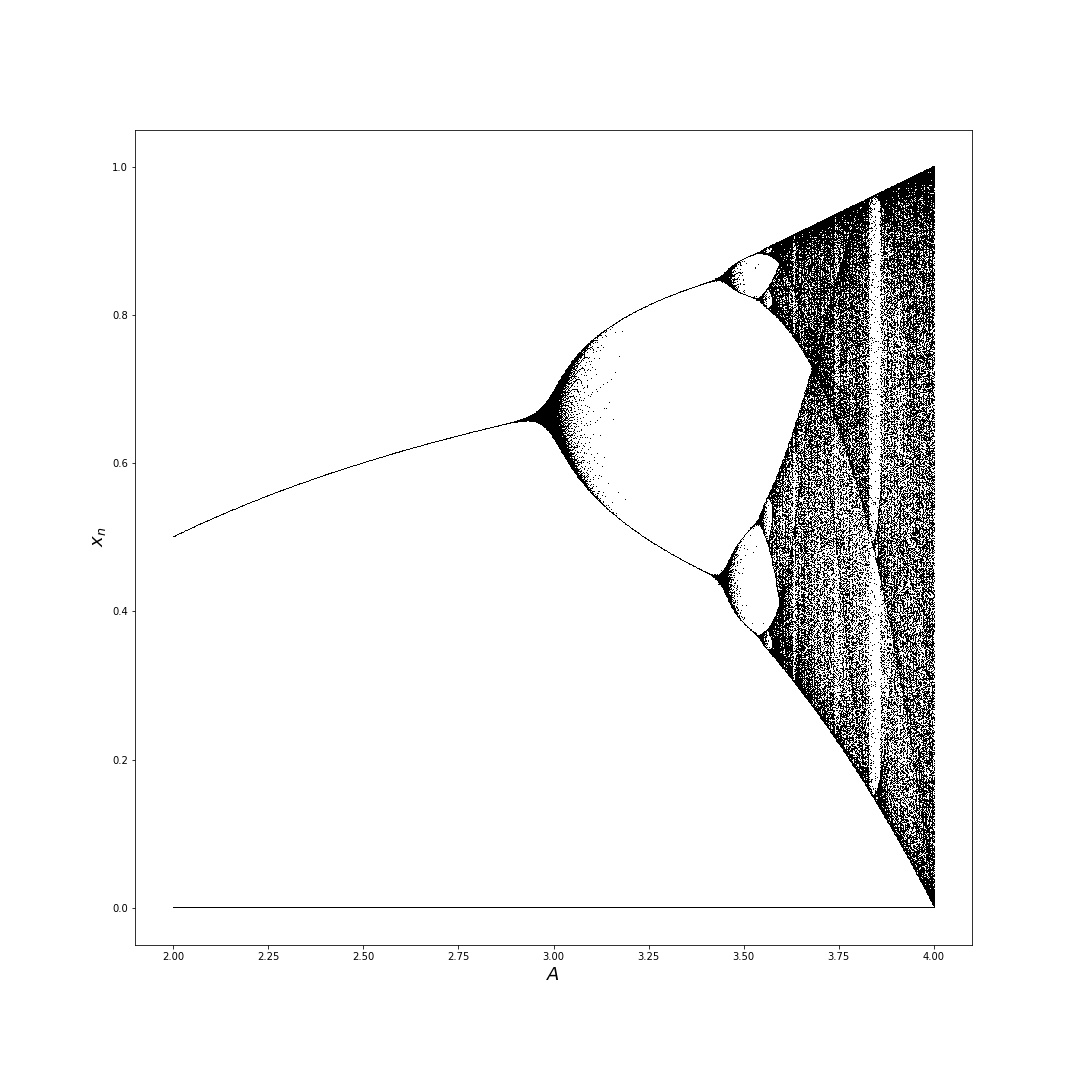
\includegraphics[width=7cm]{map_log}
\caption*{\textbf{Figura 2.2}: Representación gráfica de un mapeo de conjuntos del pelotas deportivas al conjunto de números naturales $\mathbb{N}$ }
\label{etiqueta}
\end{figure}
\end{enumerate}

\section{Atractores Extraños}
Los sistemas dinámicos son en general sistema disipativo que esta sujeto a una fuerza externa que, de no ser por esta, el sistema se detendría en un determinado  tiempo. Por consecuencia de estas fuerzas externas los sistemas tienden a evolucionar a una trayectoria específica independiente las condiciones iniciales. A estos conjuntos de estados a los que converge un sistema dinámico se les llama \textit{atractor} . Un ejemplo sencillo es un oscilador armónico forzado. Este sistema comienza en una cierta posición y velocidad (que son las condiciones iniciales), el sistema, al ser disipativo por la fricción que hay con su entorno, pierde energía tiende a llegar al reposo, pero debido a una fuerza estrena que se le aplica mientras esta en movimiento se comenzara a contrarrestar la fuerza de fricción y llegara el momento en que la energía disipada será igual a la inyectada al sistema por lo que su movimiento convergerá a una trayectoria que caracteriza a un oscilador armónico sin amortiguamiento ni fuerza externa. En la figura 3.1 se muestra el espacio fase de un oscilador armónico forzado con una fuerza externa “———pon el ejemplo de la tarea 2———“

\begin{figure}[H]
\centering
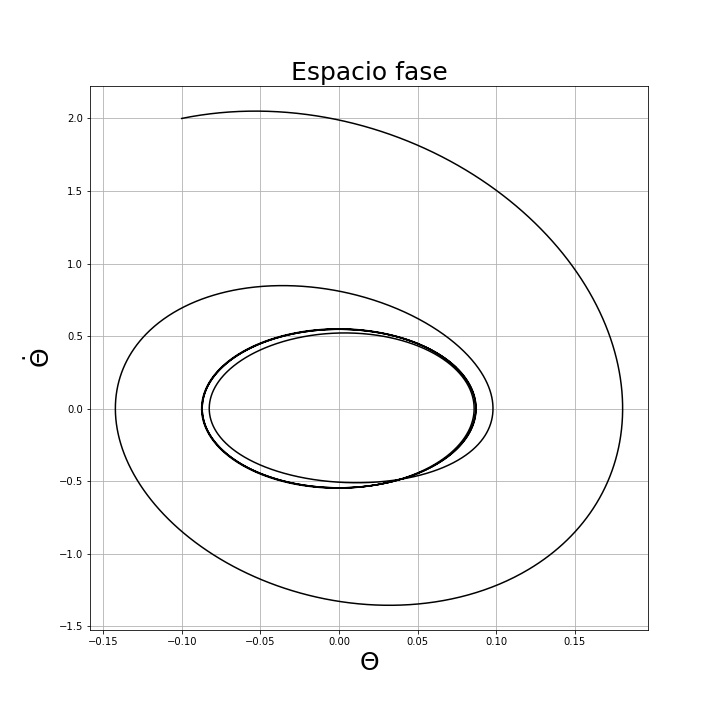
\includegraphics[width=7cm]{pendulo.jpg}
\caption*{\textbf{Figura 3.1} Espacio fase de un oscilador armónico forzado con "" }
\label{etiqueta}
\end{figure}
\end{enumerate}

Un atractor puede presentarse como un punto o como una trayectoria específica en el espacio fase del sistema dinámico. En un sistema caótico la trayectoria a la que converge el la solución tiene la forma de un fractal (En la sección de fractales se hablara más de este concepto) y se les llama \textbf{atractores extraños}. En estos casos, una vez que el sistema se encuentra en el atractor, los estados cercanos divergen entre sí de manera exponencial. Es decir, el sistema nunca vuelve al mismo lugar. El atractor más famoso en teoría de caos es el atractor de Lorenz. 

En el año 1963, el profesor Edward Lorenz(1917-2008), matemático y meteorólogo, al tratar de desarrollar un modelo matemático simple para describir la dinámica de convección atmosférica llego las siguientes tres ecuaciones:
\begin{equation} 
\begin{split} 
\frac{dx}{dt} & = a(y-x) \\
\frac{dy}{dt} & = x(b-z) - y\\
\frac{dz}{dt} & = xy-cz 
\end{split} 
\end{equation} 
Las ecuaciones describen la dinámica de un fluido con una diferencia de temperatura entre la parte superior e inferior. Donde la variable x es proporcional a la velocidad de convección y a su vez y y z son proporcionales a la variación de temperatura horizontal y vertical respectivamente. La figura 3.2 muestra la solución de forma gráfica al sistema de ecuaciones y puede observarse el conjunto continuo de estados a los que converge el sistema. 

\begin{figure}[H]
\centering
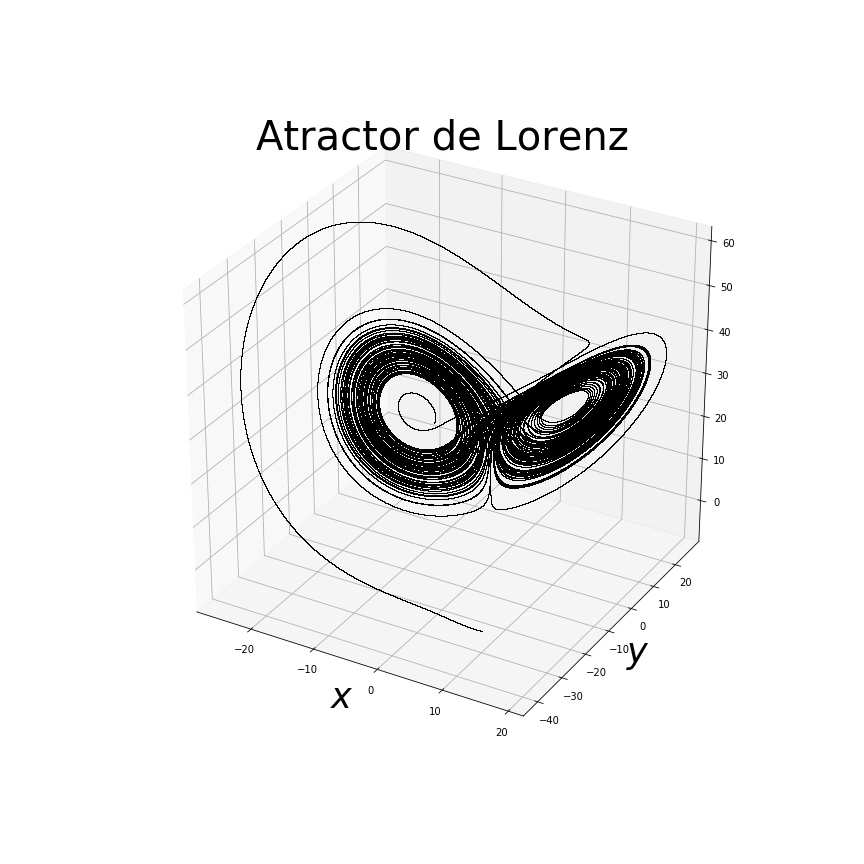
\includegraphics[width=7cm]{atrac_lor.jpg}
\caption*{\textbf{Figura 3.2} Atractor de Lorenz con parametros $a=10$, $b=28$, $c=8/3$ y condiciones iniciales $x=1$, $y=1$, $z= 1$  }
\label{etiqueta}
\end{figure}
\end{enumerate}

\section{Secciones de Poincaré}
Al estudiar los sistemas dinámicos es muy probable que se encuentren soluciones con trayectorias bastante complicadas de determinar. Para simplificar el análisis de la solución, se opta por buscar una representación de las solución sin mayor detalle a diferencia del que se muestra en el espacio fase. Las secciones de Poincaré son una herramienta útil para llevar a cabo esta tarea por medio de intersecciones perpendiculares de hiperplanos en la trayectoria que muestra la evolución del sistema.  Las secciones de Poincaré se pueden construir de forma sencilla. Tenemos un sistema dinámico:
\begin{equation}
\frac{dx}{dt} = f(x,t;\alpha) 
\end{equation}
Cuya solución describe una órbita periódica, que llamaremos $\lambda$, en un punto $x_0$ donde se construye un plano perpendicular a este. Así, para cualquier punto $x$ próximo a $x_0$ en el mismo plano perpendicular, la solución del sistema dinámico que pasa por $x$ en $t=0$, atravesará de nuevo el plano en el punto $P(x)$ próximo a $x_0$. Tenemos entonces el mapeo
\begin{equation}
\begin{split}
&P:  U \longrightarrow S \\
&x_{n} \mapsto x_{n+1} = P(x_{n})  
\end{split}
\end{equation} 
Donde U es una vecindad del punto $x$ en el plano S. A esto se le llama el mapeo, sección o aplicación de Poincaré que es presentada en 1881 por Henri Poincaré. En la figura “” se puede ver de forma gráfica la construcción del plano en una trayectoria en 3-dimenciones.

\begin{figure}[H]
\centering
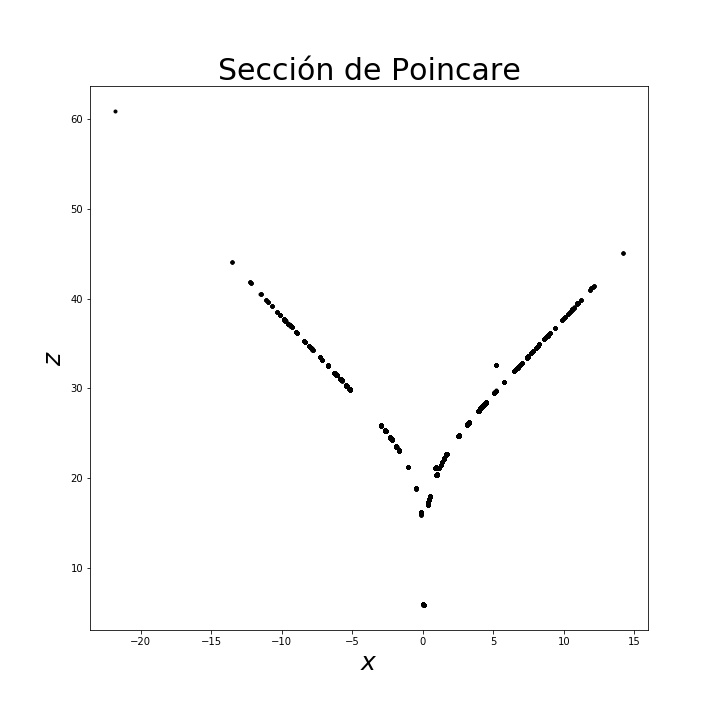
\includegraphics[width=7cm]{sec_poin.jpg}
\caption*{\textbf{Figura 4.1}  }
\label{etiqueta}
\end{figure}
\end{enumerate}

En la mayoría de casos, el mapeo de Poincaré se reduce a un mapeo iterativo unidimensional. Sin embargo, hay soluciones de sistemas que requieren de mayor información.

\subsubsection{Bibliografia}\label{sec:bio}

Más texto.

% Bibliografía.
%-----------------------------------------------------------------
\begin{thebibliography}{99}

\bibitem{Cd94} Robert C. Hilborn, \emph{Chaos and Nonlinear Dynamics: "An introduction for scientists and enginners"}, Oxford students edition, (1994) pg: 19-20

\end{thebibliography}

\end{document}